\documentclass[10pt,letterpaper]{article}
\usepackage{tools}
\usepackage{enumitem}
%\settextfont{B Nazanin}
\usepackage{lipsum}
\setlength{\parskip}{3mm}
\setlength{\parindent}{0mm}
\begin{document}
\Large
\begin{center}
In the name of beauty

1st problem set of ComNet course
\hl
\end{center}
Q1)

Determine the following statements as true or false with enough reasons.
\begin{enumerate}[label=\alph*-]
\item
False. This is the definition of propagation delay.
\item
Packet Switching is practically more complicated than Circuit Switching while being more suitable to real-time applications.
\item
False. Packet switches are also included.
\item
False. With traffic intensity being close to 1, the queuing delay of the packets tends to infinity due to packet acumulation in buffer.
\item
False. Link-layer switches are typically capable of processing the packets up to the layer 2, unless they are manipulated manually.
\item
False. SMTP and FTP are examples of layer 5 (Application Layer) protocols.
%\item
%API is a set of rules 
%\item
%For economical reasons, exploiting optical fibers is not recommended in long-haul network
\end{enumerate}
Q2)

What is the difference between \textbf{Virus} and \textbf{Worm}?

Q3)

Consider the following network in which node A wants to send packets to node B through a router and two links:
\begin{figure}[ht]
\centering
\includegraphics[width=140mm]{p2p}
\end{figure}
Assume the transmission rate of the links 1 and 2 to be 100Mbits/sec and 50Mbits/sec, respectively and both of the links be 10km long. The speed of light is $2\times 10^8$m/s in the links.
\begin{enumerate}[label=\alph*-]
\item
$$\Delta_\text{Propagation,end-to-end}=2{d\over c}=2\times{10km\over 2\times 10^5 km/s}=100\mu sec$$
\item
Since each packet is 100Kbits, it would take 1ms and 2ms for each packet to traverse the links 1 and 2 respectively. Since it is assumed for each packet to occupy a full time slot, the time slot duration is 1msec as well. By the end of the first time slot, node 1 has completed the transmission of packet 1 and heads over to hand out the packet 2. By the end of the 1st time slot (+50$\mu$sec propagation delay which is negligible), the intervening router has received packet 1 completely and immediately starts to transmit it on its link 2 interface. Since link 2 has half bit rate compared to that of link 1, the packets will take 2 time slots to pass through the link. Keeping on this track, by the end of the 4rd time slot, packets 2, 3 and 4 are received by the router, packet 1 has left the router and packet 2 is halfway through leaving the router. Hence, we end up with 2.5, yet un-transmitted, packets to be stored. The required amount of buffer capacity would then be $2.5\times 12.5=31.25$ Kbytes.
\item
Yes. Link 2 is a bottleneck for its bit rate is lower and imposes a traffic intensity of 2 on the system.
\end{enumerate}

Q4) Such a path must contain nodes A-F-G-H and two of the intermediate nodes B,C,D,E. The probability that each of the paths ABF to AEF will work, is equal to $(1-p)^2$. Since we need two of such paths, there is a probability of $\binom{4}{2}(1-p)^4[1-(1-p)^2]^2$ that a throughput of $2R$ is available between nodes A and F. Considering the path F-G-H, the probability that node A can send packets to node H would be $$\binom{4}{2}(1-p)^6[1-(1-p)^2]^2$$
\begin{figure}[ht]
\centering
\includegraphics[width=110mm]{Q5}
\end{figure}

Q5)

\begin{figure}[ht]
\centering
\includegraphics[width=140mm]{p2p_multi}
\end{figure}
\begin{enumerate}[label=\alph*-]
\item
$$
1-(1-(1-p)^2)^3
$$
\item
$$
{3(1-p)^2R}
$$
\end{enumerate}
%\noindent
%سوال 1) درستی یا نادرستی گزاره های زیر را با بیان دلایل کافی تحقیق کنید.
%
%1. برای شدت ترافیک نزدیک به $1$، تاخیر صف
%\footnote{
%\lr{Queuing delay}
%}
% بسته ها به سمت صفر میل می کند.
%
%2. داده برای انتقال از یک هاست
%\footnote{
%\lr{Host}
%}
% به هاست دیگر، فقط از مجموعه ای از لینک ها می گذرد.
%
%3. \lr{API} 
%مجموعه‌ی قوانینی است که برنامه‌ی سمت فرستنده باید پیروی کند تا اینترنت قادر به انتقال داده به برنامه‌ی مقصد باشد.
%
%4. \lr{Packet Switching}
% پیاده سازی پیچیده تر و پر هزینه تری نسبت به \lr{Circuit Switching} ایجاب می کند؛ ولی در مقابل برای کاربردهای بلادرنگ
%\footnote{
%\lr{Real-time}
%}
% مناسب تر است.
%
%5. یک پروتکل، فرمت و ترتیب پیامهای جابجاشده بین دو واحد مخابراتی را مشخص می کند و به اعمال انجام شده در ارسال و یا دریافت پیام نظارتی ندارد.
%
%6. در سمت کاربر، \lr{DSLAM} وظیفه ی جداسازی سیگنال های تلفنی و دیتای اینترنتی را در \lr{cable Internet access} بر عهده دارد.
%
%7. در معماری \lr{PON} همه ی بسته های ارسال شده از \lr{OLT} به سمت \lr{Splitter}، در \lr{Splitter} تکثیر می شوند.
%
%8. به دلایل اقتصادی، از فیبر نوری نمی توان در شبکه های \lr{long-haul} استفاده کرد.
%
%9. لایه‌ی پروتکل فقط در نرم افزار پیاده سازی می‌شود.
%
%10. تنها یک پروتکل \lr{IP} وجود دارد و تمام اجزای اینترنت که یک لایه‌ی شبکه دارند، باید از این پروتکل تبعیت کنند.
%
%\noindent
%سوال 2) تفاوت ویروس (\lr{Virus}) و کرم (\lr{Worm}) چیست؟
%
%\noindent
% سوال 3) در یک روتر، بسته
%\footnote{
%\lr{Packet}
%}
% هایی با طول 8 بیت به ورودی آن ارسال می شوند و نرخ دریافت بسته ها در ورودی از توزیع زیر پیروی می کند:
%\eqn{
%f_A(a)={(3.35)^a\cdot e^{-3.35}\over a!}
%}{}
%نرخ خروجی بیت در روتر نیز دارای توزیع زیر است:
%\eqn{
%R\sim \mathcal{U}(35,40)
%}{}
%\indent
%الف) متوسط شدت ترافیک
%\footnote{
%\lr{Traffic Intensity}
%}
% را در این روتر محاسبه کنید.
%
%\indent
%ب) اگر چهار بسته به صورت پشت سر هم وارد این روتر شوند، متوسط تاخیر ارسال
%\footnote{
%\lr{Transmission delay}
%}
% بسته‌ی چهارم چه 
%\indent
%میزان خواهد بود؟ (تاخیر ارسال بسته‌ی اول را صفر در نظر بگیرید)
%\noindent
%سوال 4) در شبکه ی زیر، اگر احتمال خرابی هر لینک مستقل از سایرین برابر $p$ باشد، احتمال صحت کل مسیر را از $A$ تا $B$ به دست آورید.
%\begin{center}
%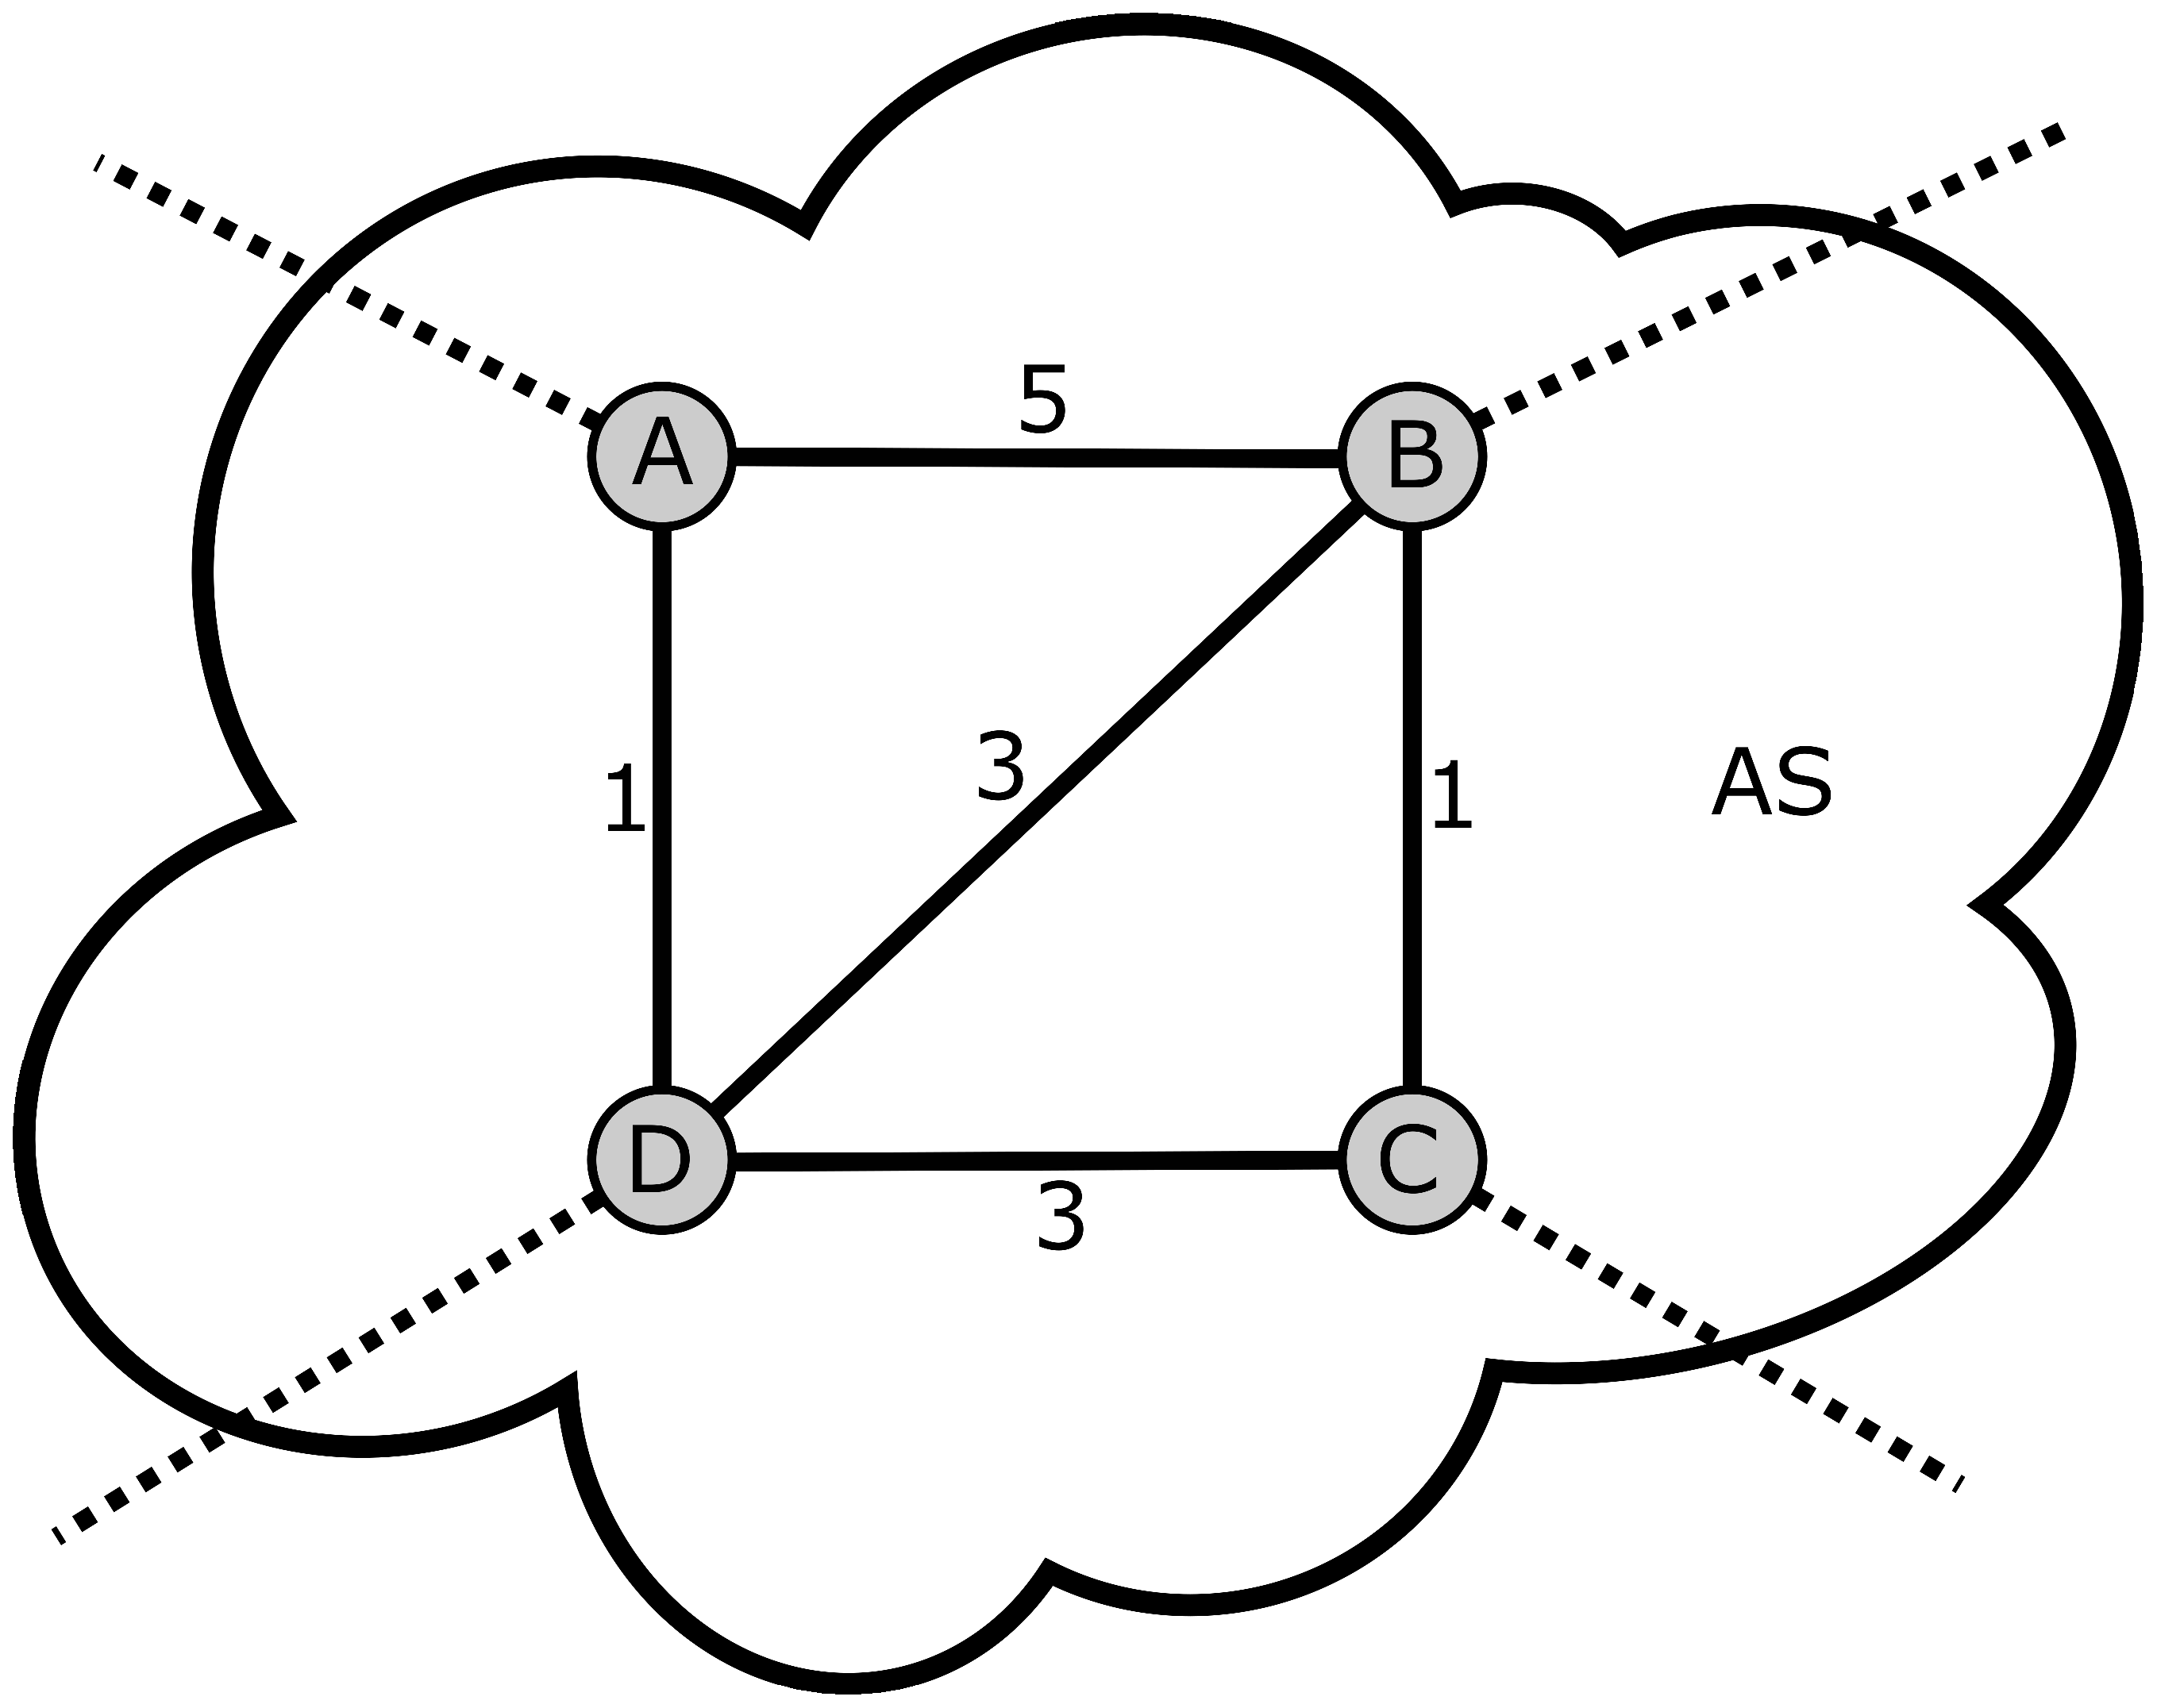
\includegraphics[width=100mm]{Q4}
%\end{center}
%سوال 5) در شبکه ای با توپولوژی زیر، در چه صورت و با کدام احتمال حداکثر \lr{throughput} برای مسیر $A-H$ برابر $2R$ می باشد؟ (احتمال خرابی هر لینک مستقل از سایرین برابر $p$ می باشد)
%\begin{center}
%\includegraphics[width=100mm]{Q5}
%\end{center}
%\noindent
%سوال 6) در شبکه‌ی زیر، فرض کنید نرخ ورود بیت به روتر برابر 
%$1\text{\lr{Mbps}}$
%، حجم هر بسته برابر 
%$1\text{\lr{kbytes}}$
%، تاخیر پردازش هر بسته برابر 
%$12\text{\lr{msec}}$
%، طول لینک برابر 200 متر و سرعت انتشار در لینک برابر 
%$2\times 10^8 \text{\lr{m/s}}$
% است. همچنین  نرخ خروج بیت از روتر را بینهایت بگیرید.
%
%الف) تاخیر ارسال را برای بسته‌ی دهم محاسبه کنید.
%
%ب) تاخیر کلی ای را که بسته‌ی دوم در ارسال از \lr{A} به \lr{B} تجربه می کند محاسبه کنید.
%
%ج) به مدت چند میلی ثانیه و برای اولین بار، حجم اشغال شده‌ی بافر برابر 
%$2\text{\lr{kbytes}}$
% خواهد بود؟ (حالتی که یک بسته بلافاصله وارد بافر می‌شود و تنها بسته‌ی کنونی بافر بلافاصله از آن خارج می‌شود، $1\text{\lr{kbytes}}$ از حجم بافر را اشغال می‌کند. به عبارت دیگر باید مدت زمان غیرصفری محاسبه شود که دو بسته همزمان در بافر حضور داشته باشند)
%\begin{center}
%\includegraphics[width=100mm]{Q6.jpg}
%\end{center}
\end{document}